% Forløbig resultater
% Opsætning
% Fuel
% Afstand
% Fremtidige tests/arbejde
% Konklusion


\section{Evaluation}
\begin{frame}{Test Setup}



\begin{columns}
	\begin{column}{0.7\textwidth}
		\begin{itemize}
		\item SUMO- Simulation of Urban MObility\\
		\item Real world road network\\
		\item Real world Traffic light phases\\
		\item Real world OD matrix\\
		\end{itemize}
	\end{column}

	\begin{column}{0.3\textwidth}
		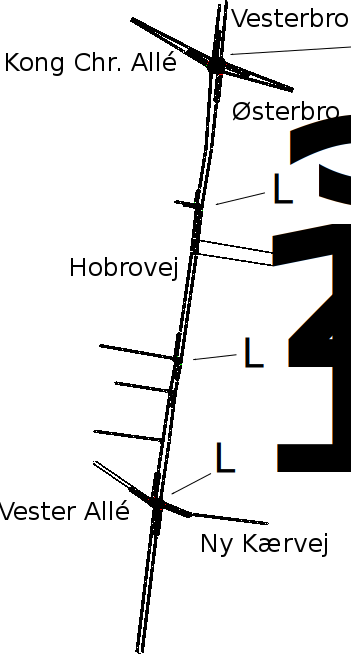
\includegraphics[width=0.8\textwidth]{images/Hobrovej.png}
	\end{column}
\end{columns}
\end{frame}

\begin{frame}{SUMO presentation}
\end{frame}

\begin{frame}{Fuelsaving}
	\begin{figure}
	\begin{tikzpicture}[scale=0.6]
	\begin{axis}[xlabel=Routes,xticklabel=\empty,ylabel=Fuel consumption,bar width=1pt,]
	\addplot[ybar, blue] table[x=Route,y=Fuel] {TestResults/0/avg.dat};
	\addplot[ybar, red] table[x=Route,y=Fuel] {TestResults/100/avg.dat};
	\draw[thick, red] (axis cs:0,138) -- (axis cs:109,138);
	\draw[thick, blue] (axis cs:0,162) -- (axis cs:109,162);
	\end{axis}
	\end{tikzpicture}
	\caption{Average fuel consumption with (red) and without \tech (blue)}\label{tik:fuel:avg}
	\end{figure}
\end{frame}


\begin{frame}{Distance}



\begin{columns}
	\begin{column}{0.5\textwidth}
	
\begin{figure}
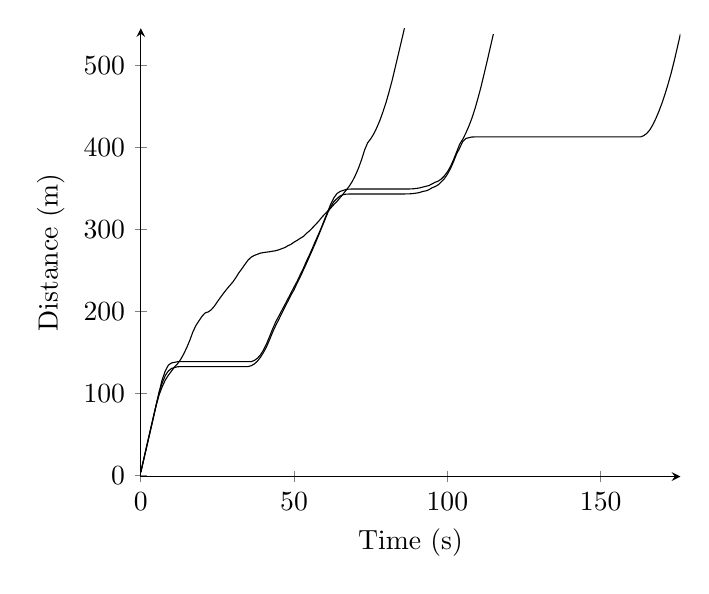
\begin{tikzpicture}
\begin{axis}[
legend style={anchor=west},
axis x line=bottom,
axis y line=left,
ymin=-1,
xlabel=Time (s),
ylabel=Distance (m),
]
\addplot[] coordinates {
(0, 4.1)
(1, 20.6645116726)
(2, 37.2233909873)
(3, 53.6521603191)
(4, 69.7829428487)
(5, 86.1531519791)
(6, 101.667779946)
(7, 113.082049876)
(8, 122.080502823)
(9, 127.572369863)
(10, 130.591078072)
(11, 131.749428121)
(12, 132.706019128)
(13, 132.881539267)
(14, 132.920666884)
(15, 132.930793993)
(16, 132.930793993)
(17, 132.930793993)
(18, 132.930793993)
(19, 132.930793993)
(20, 132.930793993)
(21, 132.930793993)
(22, 132.930793993)
(23, 132.930793993)
(24, 132.930793993)
(25, 132.930793993)
(26, 132.930793993)
(27, 132.930793993)
(28, 132.930793993)
(29, 132.930793993)
(30, 132.930793993)
(31, 132.930793993)
(32, 132.930793993)
(33, 132.930793993)
(34, 132.930793993)
(35, 132.930793993)
(36, 133.950245124)
(37, 136.038783655)
(38, 139.338817879)
(39, 144.043252469)
(40, 149.996507492)
(41, 156.893946835)
(42, 165.563489112)
(43, 174.714518179)
(44, 182.910481045)
(45, 190.161962998)
(46, 197.951793277)
(47, 205.310238155)
(48, 212.637208535)
(49, 220.112257728)
(50, 226.5629698)
(51, 234.78046901)
(52, 241.995329923)
(53, 250.259094644)
(54, 258.342745392)
(55, 266.742235195)
(56, 275.2123866)
(57, 283.8097772)
(58, 292.835265533)
(59, 302.161077436)
(60, 311.074390021)
(61, 320.419549613)
(62, 327.855001802)
(63, 333.920116456)
(64, 337.601388016)
(65, 340.651296831)
(66, 342.381063437)
(67, 342.945328569)
(68, 343.116326497)
(69, 343.161072883)
(70, 343.183898349)
(71, 343.183898349)
(72, 343.183898349)
(73, 343.183898349)
(74, 343.183898349)
(75, 343.183898349)
(76, 343.183898349)
(77, 343.183898349)
(78, 343.183898349)
(79, 343.183898349)
(80, 343.183898349)
(81, 343.183898349)
(82, 343.183898349)
(83, 343.183898349)
(84, 343.183898349)
(85, 343.183898349)
(86, 343.183898349)
(87, 343.258079659)
(88, 343.402007627)
(89, 343.769113181)
(90, 344.287095415)
(91, 345.01538894)
(92, 346.257393257)
(93, 346.92903699)
(94, 348.411688322)
(95, 350.733056157)
(96, 352.137246736)
(97, 354.299587343)
(98, 357.814834789)
(99, 361.701437318)
(100, 367.215965926)
(101, 374.005645735)
(102, 382.409629841)
(103, 391.956922395)
(104, 398.959295075)
(105, 407.005651629)
(106, 410.708245768)
(107, 411.747030177)
(108, 412.573976498)
(109, 412.643706469)
(110, 412.653102598)
(111, 412.653102598)
(112, 412.653102598)
(113, 412.653102598)
(114, 412.653102598)
(115, 412.653102598)
(116, 412.653102598)
(117, 412.653102598)
(118, 412.653102598)
(119, 412.653102598)
(120, 412.653102598)
(121, 412.653102598)
(122, 412.653102598)
(123, 412.653102598)
(124, 412.653102598)
(125, 412.653102598)
(126, 412.653102598)
(127, 412.653102598)
(128, 412.653102598)
(129, 412.653102598)
(130, 412.653102598)
(131, 412.653102598)
(132, 412.653102598)
(133, 412.653102598)
(134, 412.653102598)
(135, 412.653102598)
(136, 412.653102598)
(137, 412.653102598)
(138, 412.653102598)
(139, 412.653102598)
(140, 412.653102598)
(141, 412.653102598)
(142, 412.653102598)
(143, 412.653102598)
(144, 412.653102598)
(145, 412.653102598)
(146, 412.653102598)
(147, 412.653102598)
(148, 412.653102598)
(149, 412.653102598)
(150, 412.653102598)
(151, 412.653102598)
(152, 412.653102598)
(153, 412.653102598)
(154, 412.653102598)
(155, 412.653102598)
(156, 412.653102598)
(157, 412.653102598)
(158, 412.653102598)
(159, 412.653102598)
(160, 412.653102598)
(161, 412.653102598)
(162, 412.653102598)
(163, 412.653102598)
(164, 414.126797325)
(165, 416.762522374)
(166, 421.167417972)
(167, 427.342459388)
(168, 435.149735213)
(169, 443.99346754)
(170, 453.929697655)
(171, 465.056873084)
(172, 477.399438277)
(173, 490.662208822)
(174, 505.565412341)
(175, 521.61422612)
(176, 538.013766331)
};
\addplot[] coordinates {
(0, 4.1)
(1, 20.1645756991)
(2, 36.4586941584)
(3, 52.8995375674)
(4, 69.3520150779)
(5, 85.5253012058)
(6, 102.041913142)
(7, 117.13254816)
(8, 127.666308848)
(9, 134.690683972)
(10, 137.343303204)
(11, 138.075345254)
(12, 138.872967603)
(13, 138.928608296)
(14, 138.935539303)
(15, 138.935539303)
(16, 138.935539303)
(17, 138.935539303)
(18, 138.935539303)
(19, 138.935539303)
(20, 138.935539303)
(21, 138.935539303)
(22, 138.935539303)
(23, 138.935539303)
(24, 138.935539303)
(25, 138.935539303)
(26, 138.935539303)
(27, 138.935539303)
(28, 138.935539303)
(29, 138.935539303)
(30, 138.935539303)
(31, 138.935539303)
(32, 138.935539303)
(33, 138.935539303)
(34, 138.935539303)
(35, 138.935539303)
(36, 138.935539303)
(37, 140.361940724)
(38, 142.918385312)
(39, 147.047718442)
(40, 152.930798897)
(41, 160.478566105)
(42, 169.459154157)
(43, 178.754790064)
(44, 187.311108754)
(45, 194.261086455)
(46, 201.383695953)
(47, 208.31445685)
(48, 215.473489398)
(49, 222.722541333)
(50, 229.862697911)
(51, 236.824858315)
(52, 244.751313549)
(53, 252.378532402)
(54, 261.029446141)
(55, 268.989023324)
(56, 277.281014512)
(57, 286.183793225)
(58, 294.398021084)
(59, 303.044236257)
(60, 312.735560811)
(61, 321.830406504)
(62, 331.20831249)
(63, 338.572153188)
(64, 343.709136103)
(65, 346.190454301)
(66, 347.559712736)
(67, 348.713743847)
(68, 349.143323204)
(69, 349.171446431)
(70, 349.184130015)
(71, 349.184130015)
(72, 349.184130015)
(73, 349.184130015)
(74, 349.184130015)
(75, 349.184130015)
(76, 349.184130015)
(77, 349.184130015)
(78, 349.184130015)
(79, 349.184130015)
(80, 349.184130015)
(81, 349.184130015)
(82, 349.184130015)
(83, 349.184130015)
(84, 349.184130015)
(85, 349.184130015)
(86, 349.184130015)
(87, 349.184130015)
(88, 349.32146669)
(89, 349.534857882)
(90, 350.005338981)
(91, 350.589450792)
(92, 351.597520776)
(93, 352.50013659)
(94, 353.443800884)
(95, 355.452324523)
(96, 357.40535143)
(97, 358.765165831)
(98, 361.375204588)
(99, 365.165049749)
(100, 370.044294232)
(101, 376.609519974)
(102, 384.798549669)
(103, 394.195879853)
(104, 403.789087432)
(105, 409.696984054)
(106, 417.214242507)
(107, 425.717053726)
(108, 435.526495475)
(109, 447.004413325)
(110, 460.120630207)
(111, 474.196769298)
(112, 489.779390776)
(113, 505.512142704)
(114, 521.846597307)
(115, 537.931023023)
};
\addplot[] coordinates {
(0, 4.1)
(1, 20.5056685604)
(2, 36.6903577096)
(3, 52.5858298837)
(4, 68.7914526245)
(5, 85.3336524376)
(6, 98.6348900978)
(7, 108.46407366)
(8, 116.485819581)
(9, 122.458179885)
(10, 127.363722629)
(11, 132.482395376)
(12, 136.372787732)
(13, 141.637652116)
(14, 148.21364432)
(15, 156.068581137)
(16, 164.990451597)
(17, 175.210271389)
(18, 183.067317969)
(19, 188.809572641)
(20, 194.275069984)
(21, 198.326236264)
(22, 199.49203539)
(23, 202.213950972)
(24, 206.495253705)
(25, 211.947012774)
(26, 217.234720053)
(27, 222.318346531)
(28, 227.050322165)
(29, 231.519943993)
(30, 235.81814982)
(31, 241.213997069)
(32, 247.201266728)
(33, 252.198455075)
(34, 257.579442401)
(35, 262.61798516)
(36, 266.192948208)
(37, 268.262361864)
(38, 269.681721169)
(39, 271.118328519)
(40, 271.78801277)
(41, 272.309233711)
(42, 272.79300384)
(43, 273.477574092)
(44, 274.0370493)
(45, 275.159156249)
(46, 276.551393226)
(47, 277.925023404)
(48, 280.148926911)
(49, 281.835032947)
(50, 284.532208776)
(51, 286.705143967)
(52, 289.144000568)
(53, 291.331614292)
(54, 294.987185943)
(55, 298.146634163)
(56, 301.950977585)
(57, 305.865179662)
(58, 309.894877824)
(59, 314.613987832)
(60, 318.611992198)
(61, 322.494930591)
(62, 326.187894039)
(63, 330.384190186)
(64, 334.021180752)
(65, 338.653095942)
(66, 343.149192337)
(67, 347.933900467)
(68, 352.6493226)
(69, 358.601982088)
(70, 365.949912059)
(71, 374.514318604)
(72, 384.830386119)
(73, 396.707218525)
(74, 405.535438993)
(75, 410.356950536)
(76, 416.403901568)
(77, 424.135809567)
(78, 432.951829382)
(79, 443.294175918)
(80, 454.674150281)
(81, 467.752303182)
(82, 481.826811694)
(83, 497.449551992)
(84, 513.279509493)
(85, 529.145963489)
(86, 545.045145867)
};

\end{axis}
\end{tikzpicture}
\label{tik:distance:0:54}
\caption{0 percent diving with GSC on route $54$}
\end{figure}

	\end{column}

	\begin{column}{0.5\textwidth}
	
\begin{figure}
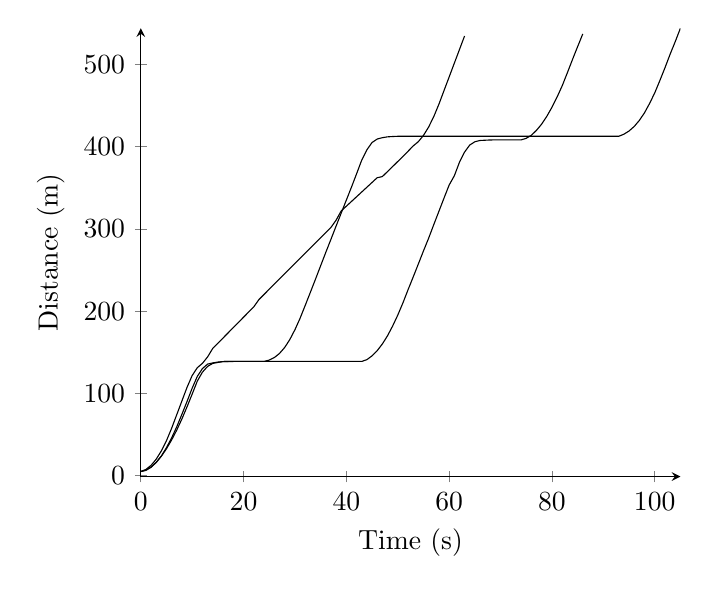
\begin{tikzpicture}
\begin{axis}[
legend style={
	anchor=west
},
axis x line=bottom,
axis y line=left,
ymin=-1,
point meta=explicit symbolic,
xlabel=Time (s),
ylabel=Distance (m)
]
\addplot[] coordinates {
(0, 5.1)
(1, 7.6)
(2, 12.6)
(3, 20.1)
(4, 30.1)
(5, 42.6)
(6, 57.6)
(7, 74.2)
(8, 90.8)
(9, 107.4)
(10, 121.758781889)
(11, 131.320742477)
(12, 136.609280481)
(13, 144.397818486)
(14, 154.68635649)
(15, 161.021784205)
(16, 167.357487819)
(17, 173.693488531)
(18, 180.029809771)
(19, 186.366477498)
(20, 192.703520555)
(21, 199.040971076)
(22, 205.378864977)
(23, 214.216758878)
(24, 220.474798436)
(25, 226.732975077)
(26, 232.991302485)
(27, 239.24979623)
(28, 245.508474103)
(29, 251.76735653)
(30, 258.026467073)
(31, 264.285833063)
(32, 270.54548638)
(33, 276.805464446)
(34, 283.065811483)
(35, 289.326580132)
(36, 295.58783356)
(37, 301.849648237)
(38, 310.611462913)
(39, 321.873277589)
(40, 327.639455454)
(41, 333.40702523)
(42, 339.176282693)
(43, 344.947614137)
(44, 350.721534016)
(45, 356.498743209)
(46, 362.280222462)
(47, 363.607388781)
(48, 369.687974655)
(49, 375.790220913)
(50, 381.925195852)
(51, 388.113297227)
(52, 394.397230867)
(53, 400.887229602)
(54, 406.011673174)
(55, 413.636116745)
(56, 423.760560316)
(57, 436.385003888)
(58, 451.509447459)
(59, 468.109447459)
(60, 484.709447459)
(61, 501.309447459)
(62, 517.909447459)
(63, 534.509447459)
};
\addplot[] coordinates {
(0, 5.1)
(1, 6.72319098396)
(2, 10.3468733498)
(3, 16.1332685505)
(4, 23.9286882805)
(5, 34.1720166711)
(6, 45.8890593831)
(7, 59.528275984)
(8, 74.6547246313)
(9, 90.2617056908)
(10, 106.406079189)
(11, 120.752868035)
(12, 130.281439818)
(13, 135.692922631)
(14, 137.147873208)
(15, 138.151456947)
(16, 138.752549833)
(17, 138.919508134)
(18, 138.930273837)
(19, 138.930273837)
(20, 138.930273837)
(21, 138.930273837)
(22, 138.930273837)
(23, 138.930273837)
(24, 138.930273837)
(25, 138.930273837)
(26, 138.930273837)
(27, 138.930273837)
(28, 138.930273837)
(29, 138.930273837)
(30, 138.930273837)
(31, 138.930273837)
(32, 138.930273837)
(33, 138.930273837)
(34, 138.930273837)
(35, 138.930273837)
(36, 138.930273837)
(37, 138.930273837)
(38, 138.930273837)
(39, 138.930273837)
(40, 138.930273837)
(41, 138.930273837)
(42, 138.930273837)
(43, 138.930273837)
(44, 141.114915808)
(45, 145.723578326)
(46, 151.998746932)
(47, 160.122800526)
(48, 170.022035583)
(49, 181.88207967)
(50, 195.182643297)
(51, 209.951444677)
(52, 226.009298917)
(53, 241.535058473)
(54, 257.259677345)
(55, 273.192092192)
(56, 288.571607169)
(57, 305.072725588)
(58, 321.279140443)
(59, 337.433303376)
(60, 353.346931963)
(61, 364.463502929)
(62, 380.895988341)
(63, 393.376922659)
(64, 401.949110189)
(65, 405.94426858)
(66, 407.522011955)
(67, 407.847468212)
(68, 408.163202868)
(69, 408.195381563)
(70, 408.195381563)
(71, 408.195381563)
(72, 408.195381563)
(73, 408.195381563)
(74, 408.195381563)
(75, 410.18501972)
(76, 413.845617016)
(77, 419.917654902)
(78, 427.393386755)
(79, 436.836262111)
(80, 447.819760421)
(81, 460.280904293)
(82, 474.035882427)
(83, 489.7969413)
(84, 505.936939978)
(85, 521.577093631)
(86, 537.018117137)
};
\addplot[] coordinates {
(0, 5.1)
(1, 6.52942920473)
(2, 10.397460774)
(3, 16.2332625509)
(4, 23.6898428533)
(5, 32.7746166262)
(6, 43.4439596056)
(7, 55.4796695473)
(8, 68.9530208007)
(9, 83.7525044986)
(10, 99.1987196739)
(11, 115.018047915)
(12, 125.904988034)
(13, 132.893465407)
(14, 136.539717246)
(15, 137.713754698)
(16, 138.775338083)
(17, 138.887378187)
(18, 138.919642787)
(19, 138.937871182)
(20, 138.937871182)
(21, 138.937871182)
(22, 138.937871182)
(23, 138.937871182)
(24, 138.937871182)
(25, 140.600580891)
(26, 143.690544118)
(27, 148.673520683)
(28, 155.907791651)
(29, 165.526496226)
(30, 177.544292589)
(31, 191.406263769)
(32, 207.110921725)
(33, 222.961991482)
(34, 239.000783121)
(35, 255.251148179)
(36, 271.513491617)
(37, 287.341622586)
(38, 303.408023612)
(39, 319.255356152)
(40, 335.112647816)
(41, 350.841227009)
(42, 367.19319554)
(43, 383.738226039)
(44, 396.198486332)
(45, 405.06887588)
(46, 409.280332872)
(47, 410.942766083)
(48, 411.946804448)
(49, 412.338587013)
(50, 412.617241737)
(51, 412.658060886)
(52, 412.658060886)
(53, 412.658060886)
(54, 412.658060886)
(55, 412.658060886)
(56, 412.658060886)
(57, 412.658060886)
(58, 412.658060886)
(59, 412.658060886)
(60, 412.658060886)
(61, 412.658060886)
(62, 412.658060886)
(63, 412.658060886)
(64, 412.658060886)
(65, 412.658060886)
(66, 412.658060886)
(67, 412.658060886)
(68, 412.658060886)
(69, 412.658060886)
(70, 412.658060886)
(71, 412.658060886)
(72, 412.658060886)
(73, 412.658060886)
(74, 412.658060886)
(75, 412.658060886)
(76, 412.658060886)
(77, 412.658060886)
(78, 412.658060886)
(79, 412.658060886)
(80, 412.658060886)
(81, 412.658060886)
(82, 412.658060886)
(83, 412.658060886)
(84, 412.658060886)
(85, 412.658060886)
(86, 412.658060886)
(87, 412.658060886)
(88, 412.658060886)
(89, 412.658060886)
(90, 412.658060886)
(91, 412.658060886)
(92, 412.658060886)
(93, 412.658060886)
(94, 415.153000888)
(95, 419.023672137)
(96, 424.501100973)
(97, 431.86335141)
(98, 441.039908442)
(99, 452.511470428)
(100, 465.308069565)
(101, 480.38143179)
(102, 496.032202461)
(103, 512.437839659)
(104, 527.797351639)
(105, 543.987083911)
};

\end{axis}
\end{tikzpicture}
\label{tik:50:12_O, 13_S, 15_N, 17_S, 17_S.-60, 19_V}
\caption{50 percent diving with GSC on route $12_O, 13_S, 15_N, 17_S, 17_S.-60, 19_V$}
\end{figure}

	\end{column}
\end{columns}
\end{frame}